
%(BEGIN_QUESTION)
% Copyright 2010, Tony R. Kuphaldt, released under the Creative Commons Attribution License (v 1.0)
% This means you may do almost anything with this work of mine, so long as you give me proper credit

Three redundant temperature transmitters measure the same point at the top of this chemical reactor vessel, with their respective signals connected to analog input channels on a SIS logic solver (``safety PLC'').  Their purpose is to detect a high-temperature condition inside the reactor, prompting shutdown logic to bring the chemical reaction to a safe temperature without any need for human operator intervention:

$$\includegraphics[width=15.5cm]{i04751x01.eps}$$

Inside the logic solver, the three transmitters' signals are ``voted'' on using a {\it median select} function block, and the selected transmitter signal is then compared against the high-temperature trip value by the shutdown logic functions.  

Based on this description of the high-temperature safety instrumented function (SIF), determine the ``MooN'' designations for the three temperature transmitters, both from the perspective of dependability (shutting down the reactor) and from the perspective of security (being able to operate):

\vskip 10pt

MooN (dependability) = \underbar{\hskip 50pt}  \hskip 70pt MooN (security) = \underbar{\hskip 50pt}

\underbar{file i04751}
%(END_QUESTION)





%(BEGIN_ANSWER)

MooN (dependability) = \underbar{\bf 2oo3}  \hskip 70pt MooN (security) = \underbar{\bf 2oo3}

%(END_ANSWER)





%(BEGIN_NOTES)

{\bf This question is intended for exams only and not worksheets!}

%(END_NOTES)


